\documentclass[notes,aspectratio=169]{beamer}
\usepackage{pgfpages}
% shared import of packages and command definitions for slides and text

\usepackage{epsfig} % Allows the inclusion of eps files
\usepackage{epic} % Enhanced picture mode
\usepackage{eepic} % Extensions for epic
\usepackage{url} % URL handling
\usepackage{longtable} % Tables that continue onto multiple pages
\usepackage{mathrsfs} % Support for \mathscr script
\usepackage{multirow} % Span rows in tables
\usepackage{bigstrut} % Space struts in tables up and down
\usepackage{amssymb} % AMS math symbols and helpers
\usepackage{graphicx} % Enhanced graphics support
\usepackage{setspace} % Adjust spacing in captions, single by default
\usepackage{xspace} % Automatically adjusting space after macros
\usepackage{amsmath} % \text, and other math formatting options
\usepackage{siunitx} % \num{} formatting and SI unit formatting
\usepackage{booktabs} % Enhanced tables with \toprule, etc.
\usepackage{hyperref} % Add clickable links to other parts of the document
\usepackage{subcaption}
\usepackage{graphicx} % Allows including images

\usepackage[noabbrev,capitalise]{cleveref} % Automatically determine \cref type

% Configure the cleveref package
\newcommand{\creflastconjunction}{, and } % Always use the serial comma

\usepackage[compat=1.1.0]{tikz-feynman} % for feynman diagrams
\tikzfeynmanset{
    warn luatex = {false}
}

\usepackage{hepunits}
% Configure the siunitx package
\sisetup{
    group-separator = {,}, % Use , to separate groups of digits, like 12,345
    list-final-separator = {, and } % Always use the serial comma in \SIlist
}

\newcommand{\fourgev}{\qty{4}{GeV}\xspace}
\newcommand{\eightgev}{\qty{8}{GeV}\xspace}
\newcommand{\ecal}{ECal}
\newcommand{\hcal}{HCal}

\usepackage{acronym}
\acrodef{dm}[DM]{Dark Matter}
\acrodef{sm}[SM]{Standard Model}
\acrodef{gr}[GR]{General Relativity}
\acrodef{cmb}[CMB]{Cosmic Microwave Background}
\acrodef{bao}[BAO]{Baryon Acoustic Oscillations}
\acrodef{hep}[HEP]{High Energy Physics}
\acrodef{wimp}[WIMP]{Weakly Interacting Massive Particle}
\acrodef{ecal}[ECal]{Electromagnetic Calorimeter}
\acrodef{hcal}[HCal]{Hadronic Calorimeter}
\acrodef{ldmx}[LDMX]{Light Dark Matter eXperiment}
\acrodef{hps}[HPS]{Heavy Photon Search experiment}
\acrodef{jlab}[JLab]{Thomas Jefferson National Accelerator Laboratory}
\acrodef{cebaf}[CEBAF]{Continuous Electron Beam Accelerator Facility}
\acrodef{kf}[KF]{Kalman Filter}
\acrodef{gbl}[GBL]{General Broken Lines}
\acrodef{svt}[SVT]{Silicon Vertex Tracker}
\acrodef{bdt}[BDT]{Boosted Decision Tree}
\acrodef{eot}[EoT]{Electrons on Target}
\acrodef{eat}[EaT]{\ac{ecal} as Target}
\acrodef{mm}[MM]{Missing Momentum}
\acrodef{vps}[VPS]{Vertex Projection Significance}

\def\minyzero{$y_{0,\min}$\xspace}
\def\maxyzeroerr{$\sigma_{y_0,\max}$\xspace}

%Environment for drawing on pictures using tikz
%   #1 Width to adjust image to (default: \textwidth)
%   #2 Filepath to image
%Use like:
%   \begin{tikzimage}[height]{filepath}
%       ...\draw...( coordinates are in fractions of width/height of image )
%   \end{tikzimage}
\newenvironment{tikzimage}[2][\textwidth]{%
    \begin{tikzpicture}
        \node[anchor=south west, inner sep=0] (image) at (0,0)
            {\includegraphics[width=#1]{{#2}}};
        \begin{scope}[x={(image.south east)},y={(image.north west)}]
}{%
        \end{scope}
    \end{tikzpicture}
}%


% HPS Diagrams
%   using tikz math library to name variables to helpful names
%   define command to draw boilerplate target/L1/L2
\usetikzlibrary{math}

% colors for diagram
\definecolor{HPSTarget}{rgb}{0.55,0.52,0.54}
\definecolor{HPSTracker}{rgb}{0.0,0.5,0.5}
\definecolor{HPSEcal}{rgb}{0.8,0.5,0.2}

\tikzmath{%
  \openingslope = 0.15; % y changer per x change
  \sensorsep = 0.12; % separation between sensors in a layer
  \sensorlen = 1.5; % length of sensors in vertical direction
  \targetx = -3.0;
  \layeronex = -0.2;
  \layertwox = 2.0;
  \targethalfthick = 0.1;
  \ecalbarlen=1.5;
  \ecalbarwidth=0.3;
  % can't have a blank line in this block
  %
  % compute locations
  \layeroney = (\layeronex - \targetx) * \openingslope;
  \layertwoy = (\layertwox - \targetx) * \openingslope;
  \sensorhalfsep = \sensorsep / 2;
  \reflineendx = \layertwox+0.5;
  \reflineendy = (\reflineendx - \targetx) * \openingslope;
}

\newcommand{\drawhpsfirsttwolayers}{%
  \draw[HPSTracker, very thick]
    (\layeronex-\sensorhalfsep,-\layeroney-\sensorlen)
    -- (\layeronex-\sensorhalfsep,-\layeroney)
    (\layeronex+\sensorhalfsep,-\layeroney-\sensorlen)
    -- (\layeronex+\sensorhalfsep,-\layeroney)
    (\layeronex-\sensorhalfsep,\layeroney+\sensorlen)
    -- (\layeronex-\sensorhalfsep,\layeroney)
    (\layeronex+\sensorhalfsep,\layeroney+\sensorlen)
    -- (\layeronex+\sensorhalfsep,\layeroney);
  \draw[HPSTracker] (\layeronex,\layeroney+\sensorlen) node[above] {L1};
  
  \draw[HPSTracker, very thick]
    (\layertwox-\sensorhalfsep,-\layertwoy-\sensorlen)
    -- (\layertwox-\sensorhalfsep,-\layertwoy)
    (\layertwox+\sensorhalfsep,-\layertwoy-\sensorlen)
    -- (\layertwox+\sensorhalfsep,-\layertwoy)
    (\layertwox-\sensorhalfsep,\layertwoy+\sensorlen)
    -- (\layertwox-\sensorhalfsep,\layertwoy)
    (\layertwox+\sensorhalfsep,\layertwoy+\sensorlen)
    -- (\layertwox+\sensorhalfsep,\layertwoy);
  \draw[HPSTracker] (\layertwox,\layertwoy+\sensorlen) node[above] {L2};
  
  \draw[gray,dashed] (\targetx,0) -- (\reflineendx,\reflineendy);
  \draw[gray,dashed] (\targetx,0) -- (\reflineendx,0);
  \draw[gray,dashed] (\targetx,0) -- (\reflineendx,-\reflineendy);
  
  \fill[HPSTarget] (\targetx-\targethalfthick,+1) rectangle (\targetx+\targethalfthick,-1);
  \draw[HPSTarget] (\targetx,-1) node[below] {Target};
}

\newcommand{\drawhps}{%
  \foreach \layerX/\layerY in {
    0.0/0.15,
    2.0/0.30,
    4.0/0.45,
    6.0/0.60,
    8.0/0.75,
    10.0/0.90
  }{
    \draw[HPSTracker, very thick]
      (\layerX-\sensorhalfsep,-\layerY-\sensorlen)
      -- (\layerX-\sensorhalfsep,-\layerY)
      (\layerX+\sensorhalfsep,-\layerY-\sensorlen)
      -- (\layerX+\sensorhalfsep,-\layerY)
      (\layerX-\sensorhalfsep,\layerY+\sensorlen)
      -- (\layerX-\sensorhalfsep,\layerY)
      (\layerX+\sensorhalfsep,\layerY+\sensorlen)
      -- (\layerX+\sensorhalfsep,\layerY);
  }
  \draw[HPSTracker] (9.0,0.75+\sensorlen) node[above,font=\LARGE] {SVT};

  \foreach \barY in {
    0.9,
    1.2,
    1.5,
    1.8,
    2.1
  }{
    \draw[draw=HPSEcal,fill=HPSEcal!20!white]
      (12.0,\barY) rectangle (12+\ecalbarlen,\barY+\ecalbarwidth)
      (12.0,-\barY) rectangle (12+\ecalbarlen,-\barY-\ecalbarwidth)
    ;
  }
  \draw[HPSEcal] (12+\ecalbarlen/2,2.1+\ecalbarwidth) node[above,font=\LARGE] {ECal};

  \draw[gray,dashed] (\targetx,0) -- (12+\ecalbarlen+0.5,0);
  
  \fill[HPSTarget] (\targetx-\targethalfthick,+1) rectangle (\targetx+\targethalfthick,-1);
  \draw[HPSTarget] (\targetx,-1) node[below left,font=\LARGE] {Target};

  \node (decay) at (\targetx+1.0,0.05) [circle,fill,inner sep=1.5pt] {};
  \node (production) at (\targetx,0.0) [circle,fill,inner sep=1.5pt] {};

  \draw[black,very thick,->]
    (\targetx-1.5,0.0) node[anchor=south east,font=\Large] {\(e^-\)} -- (\targetx-0.2,0.0);
  \draw[black,very thick,->]
    (decay) -- (11.8,1.6) node[anchor=south east,font=\Large] {\(e^-\)};
  \draw[black,very thick,->]
    (decay) -- (11.8,-2.2) node[anchor=north east,font=\Large] {\(e^+\)};
  \draw[black,very thick,->]
    (production) -- (-1.0,-0.5-\sensorlen) node[anchor=east,font=\Large] {\(e^-\)};

  \draw[blue,thick,->] (production) -- (decay) node[midway,above,font=\Large] {\(V_D\)};
}


\mode<presentation> {
  \usetheme{Madrid}

  \addtobeamertemplate{frametitle}{}{
      \begin{textblock*}{100mm}(0.8\textwidth,-0.95cm)
          
\includegraphics[height=0.95cm]{ldmx_logo}
      \end{textblock*}
      \begin{textblock*}{100mm}(0.7\textwidth,-0.95cm)
        
\includegraphics[height=0.95cm]{heavy_photon_logo}
      \end{textblock*}
  }

  \setbeamercolor{structure}{fg = UMNStormy }

  \setbeamercolor{palette primary}{fg = UMNMaroon, bg = UMNLightGray}
  \setbeamercolor{palette secondary}{fg = UMNMaroon, bg = white }
  \setbeamercolor{palette tertiary}{fg = UMNLightGold, bg = UMNStormy}

  \setbeamercolor{frametitle}{fg = UMNLightGold, bg = UMNMaroon }
  \setbeamercolor{title}{fg = UMNMaroon, bg = UMNLightGray }

  \setbeamercolor{section in toc}{fg = UMNMaroon}
  \setbeamercolor{section in toc shaded}{fg = UMNMaroon}
  
  \setbeamercolor{button}{fg = UMNLightGold, bg = UMNMaroon }
  
  \setbeamercolor{palette sidebar secondary}{fg = UMNMaroon }
  \setbeamercolor{section in sidebar shaded}{fg = UMNMaroon }

  \setbeamertemplate{itemize item}{\color{UMNMaroon}$\blacksquare$}
  \setbeamertemplate{itemize subitem}{\color{UMNLightGold}$\blacktriangleright$}
  \setbeamertemplate{enumerate items}[default]
  \setbeamertemplate{sections/subsections in toc}[sections numbered]

  \setbeamertemplate{navigation symbols}{} % To remove the navigation symbols from the bottom of all slides

  \setbeamercolor{block body alerted}{fg = UMNSunny, bg = UMNMaroon!20}
  \setbeamercolor{block title alerted}{fg = UMNLightGold, bg = UMNMaroon}
}

\def\with{}

\author{Tom Eichlersmith} % Your name
\institute[UMN] % Your institution as it will appear on the bottom of every slide, may be shorthand to save space
{
he/him/his \\ \medskip
University of Minnesota \\ \medskip
\href{mailto:eichl008@umn.edu}{eichl008@umn.edu} \\ \medskip
\begin{tabular}{p{0.4\textwidth}} \centering\with \end{tabular}
}



%\setbeamertemplate{note page}[plain]
%\setbeamertemplate{show notes on second screen=right}

\newcommand{\ssection}[2]{%
  \section{#1}%
  \begin{frame}[label={#2}]%
    \vfill%
    \centering%
    \begin{beamercolorbox}[sep=8pt,center,shadow=true,rounded=true]{title}%
        \usebeamerfont{title}#1\par%
    \end{beamercolorbox}%
    \vfill%
  \end{frame}%
}%

\newenvironment{sframe}[1]{%
  \subsection{#1}%
  \begin{frame}{#1}%
}{%
  \end{frame}%
}%

\title[Fixed Target Searches]{Fixed Target Searches for Dark Matter Production}

\begin{document}

\begin{frame}
  \maketitle
\end{frame}

\note[itemize]{
\item Welcome, I'll be talking about my disseration research focused
  on two fixed target experiments (HPS and LDMX) looking for the production
  of dark matter.
\item Please offer feedback -- first attempt to unify the two experiments into one talk.
\item Trying to focus on making talk cohesive
}

\begin{frame}{Outline}
  \begin{columns}
    \begin{column}{0.5\textwidth}
      \tableofcontents
    \end{column}
    \begin{column}{0.5\textwidth}
    \end{column}
  \end{columns}
\end{frame}

\note[itemize]{
\item Background to get us on the same footing and using the same vocabulary
\item Motivate category of DM that experiments are searching for
\item Go through my analyses within both experiments
}

\ssection{Background}{background}

\subsection{HEP Vocabulary}

\begin{frame}{Standard Model}
  \begin{columns}
    \begin{column}{0.4\textwidth}
      \begin{figure}
        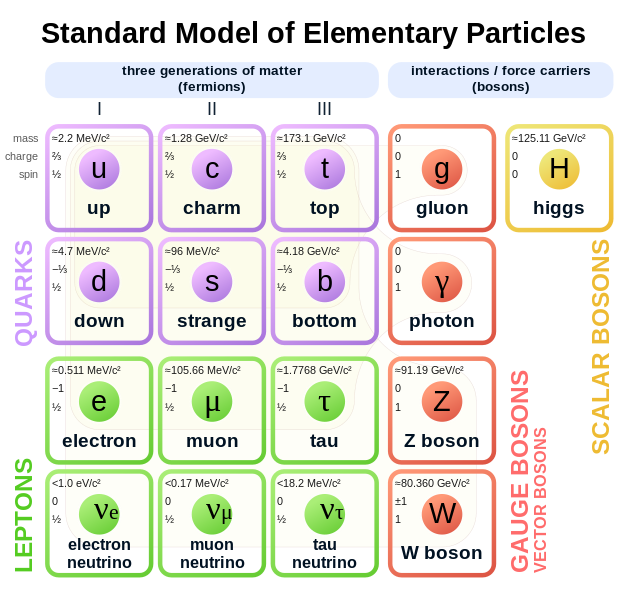
\includegraphics[width=\textwidth]{../figures/intro/Standard_Model_of_Elementary_Particles.svg.png}
        \caption{Credit to user Cush on wikipedia for providing this diagram.}
      \end{figure}
    \end{column}
    \begin{column}{0.6\textwidth}
      \begin{itemize}
        \item \boldcol{UMNSunny}{Law} -- summary of a set of consistent observations about phenomena
        \item \boldcol{UMNSunny}{Model} -- package of ``laws'' and their mathematical forms from which we can make predictions about future observations
      \end{itemize}
    \end{column}
  \end{columns}
\end{frame}

\note[itemize]{
\item Laws are summaries of observations and models
  are just packaging these laws with some mathematical sugar
\item The SM is the most quantitatively accurate physics model ever known to human kind.
\item It is a package of particles and their interactions (also represented by particles)
  from which we can -- with a specific mathematical framework -- make predictions about
  our observations.
\item \textbf{BUT} it fails to account for all observed phenomena (e.g. \emph{gravity})
}

%\begin{frame}{Feynman Diagram}
%\end{frame}
%
%\begin{frame}{Particle Mixing}
%  \begin{columns}
%    \begin{column}{0.4\textwidth}
%      \begin{figure}
%        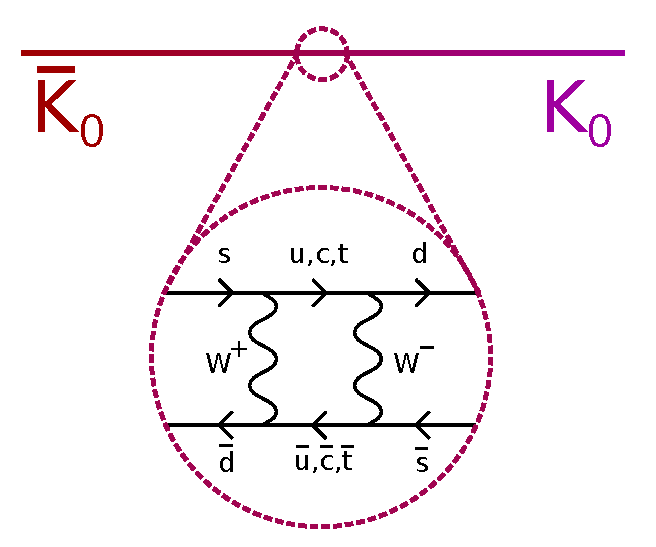
\includegraphics[width=\textwidth]{%
%          ../figures/intro/Kaon-box-diagram-with-bar.pdf%
%        }
%        \caption{Figure created by user NikNaks on Wikipedia.}
%      \end{figure}
%    \end{column}
%  \end{columns}
%\end{frame}
%
%\begin{frame}{Displaced Decay Vertices}
%  \begin{columns}
%    \begin{column}{0.5\textwidth}
%      \begin{figure}
%        \begin{tikzimage}[0.6\textwidth]{../figures/intro/bubble-chamber.jpeg}
%          \definecolor{brilliantrose}{rgb}{1.0, 0.33, 0.64}
%          % \draw[step=0.1,black,thin] (0.0,0.0) grid (1.0,1.0);
%          \node (prod) at (0.4,0.54) {};
%          \node[circle,draw=brilliantrose] (decay) at (0.515,0.54) {};
%          \draw[dashed,brilliantrose,thick] (prod) -- (decay);
%      
%          \node (beam1) at (0.1,0.5) {\color{brilliantrose}\(\pi^-\)};
%          \node (beam2) at (0.2,0.5) {};
%          \draw[->,brilliantrose,thick] (beam1) -- (beam2);
%        \end{tikzimage}
%        \caption{Image of CERN's first liquid hydrogen bubble chamber from 1960.}
%      \end{figure}
%    \end{column}
%  \end{columns}
%\end{frame}

\subsection{Dark Matter}
\begin{frame}{Dark Matter}
  \begin{columns}
    \begin{column}{0.5\textwidth}
      \begin{figure}
        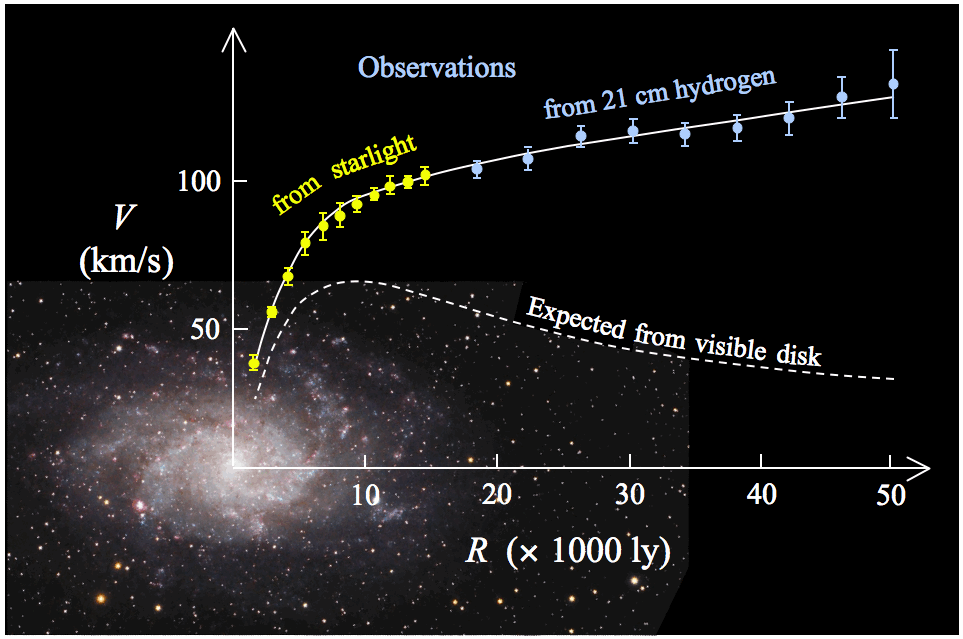
\includegraphics[width=\textwidth]{../figures/theory/rotation-curve-evidence-for-dm.png}
        \caption{Stuff is spinning too fast!}
      \end{figure}
    \end{column}
    \begin{column}{0.5\textwidth}
      \begin{figure}
        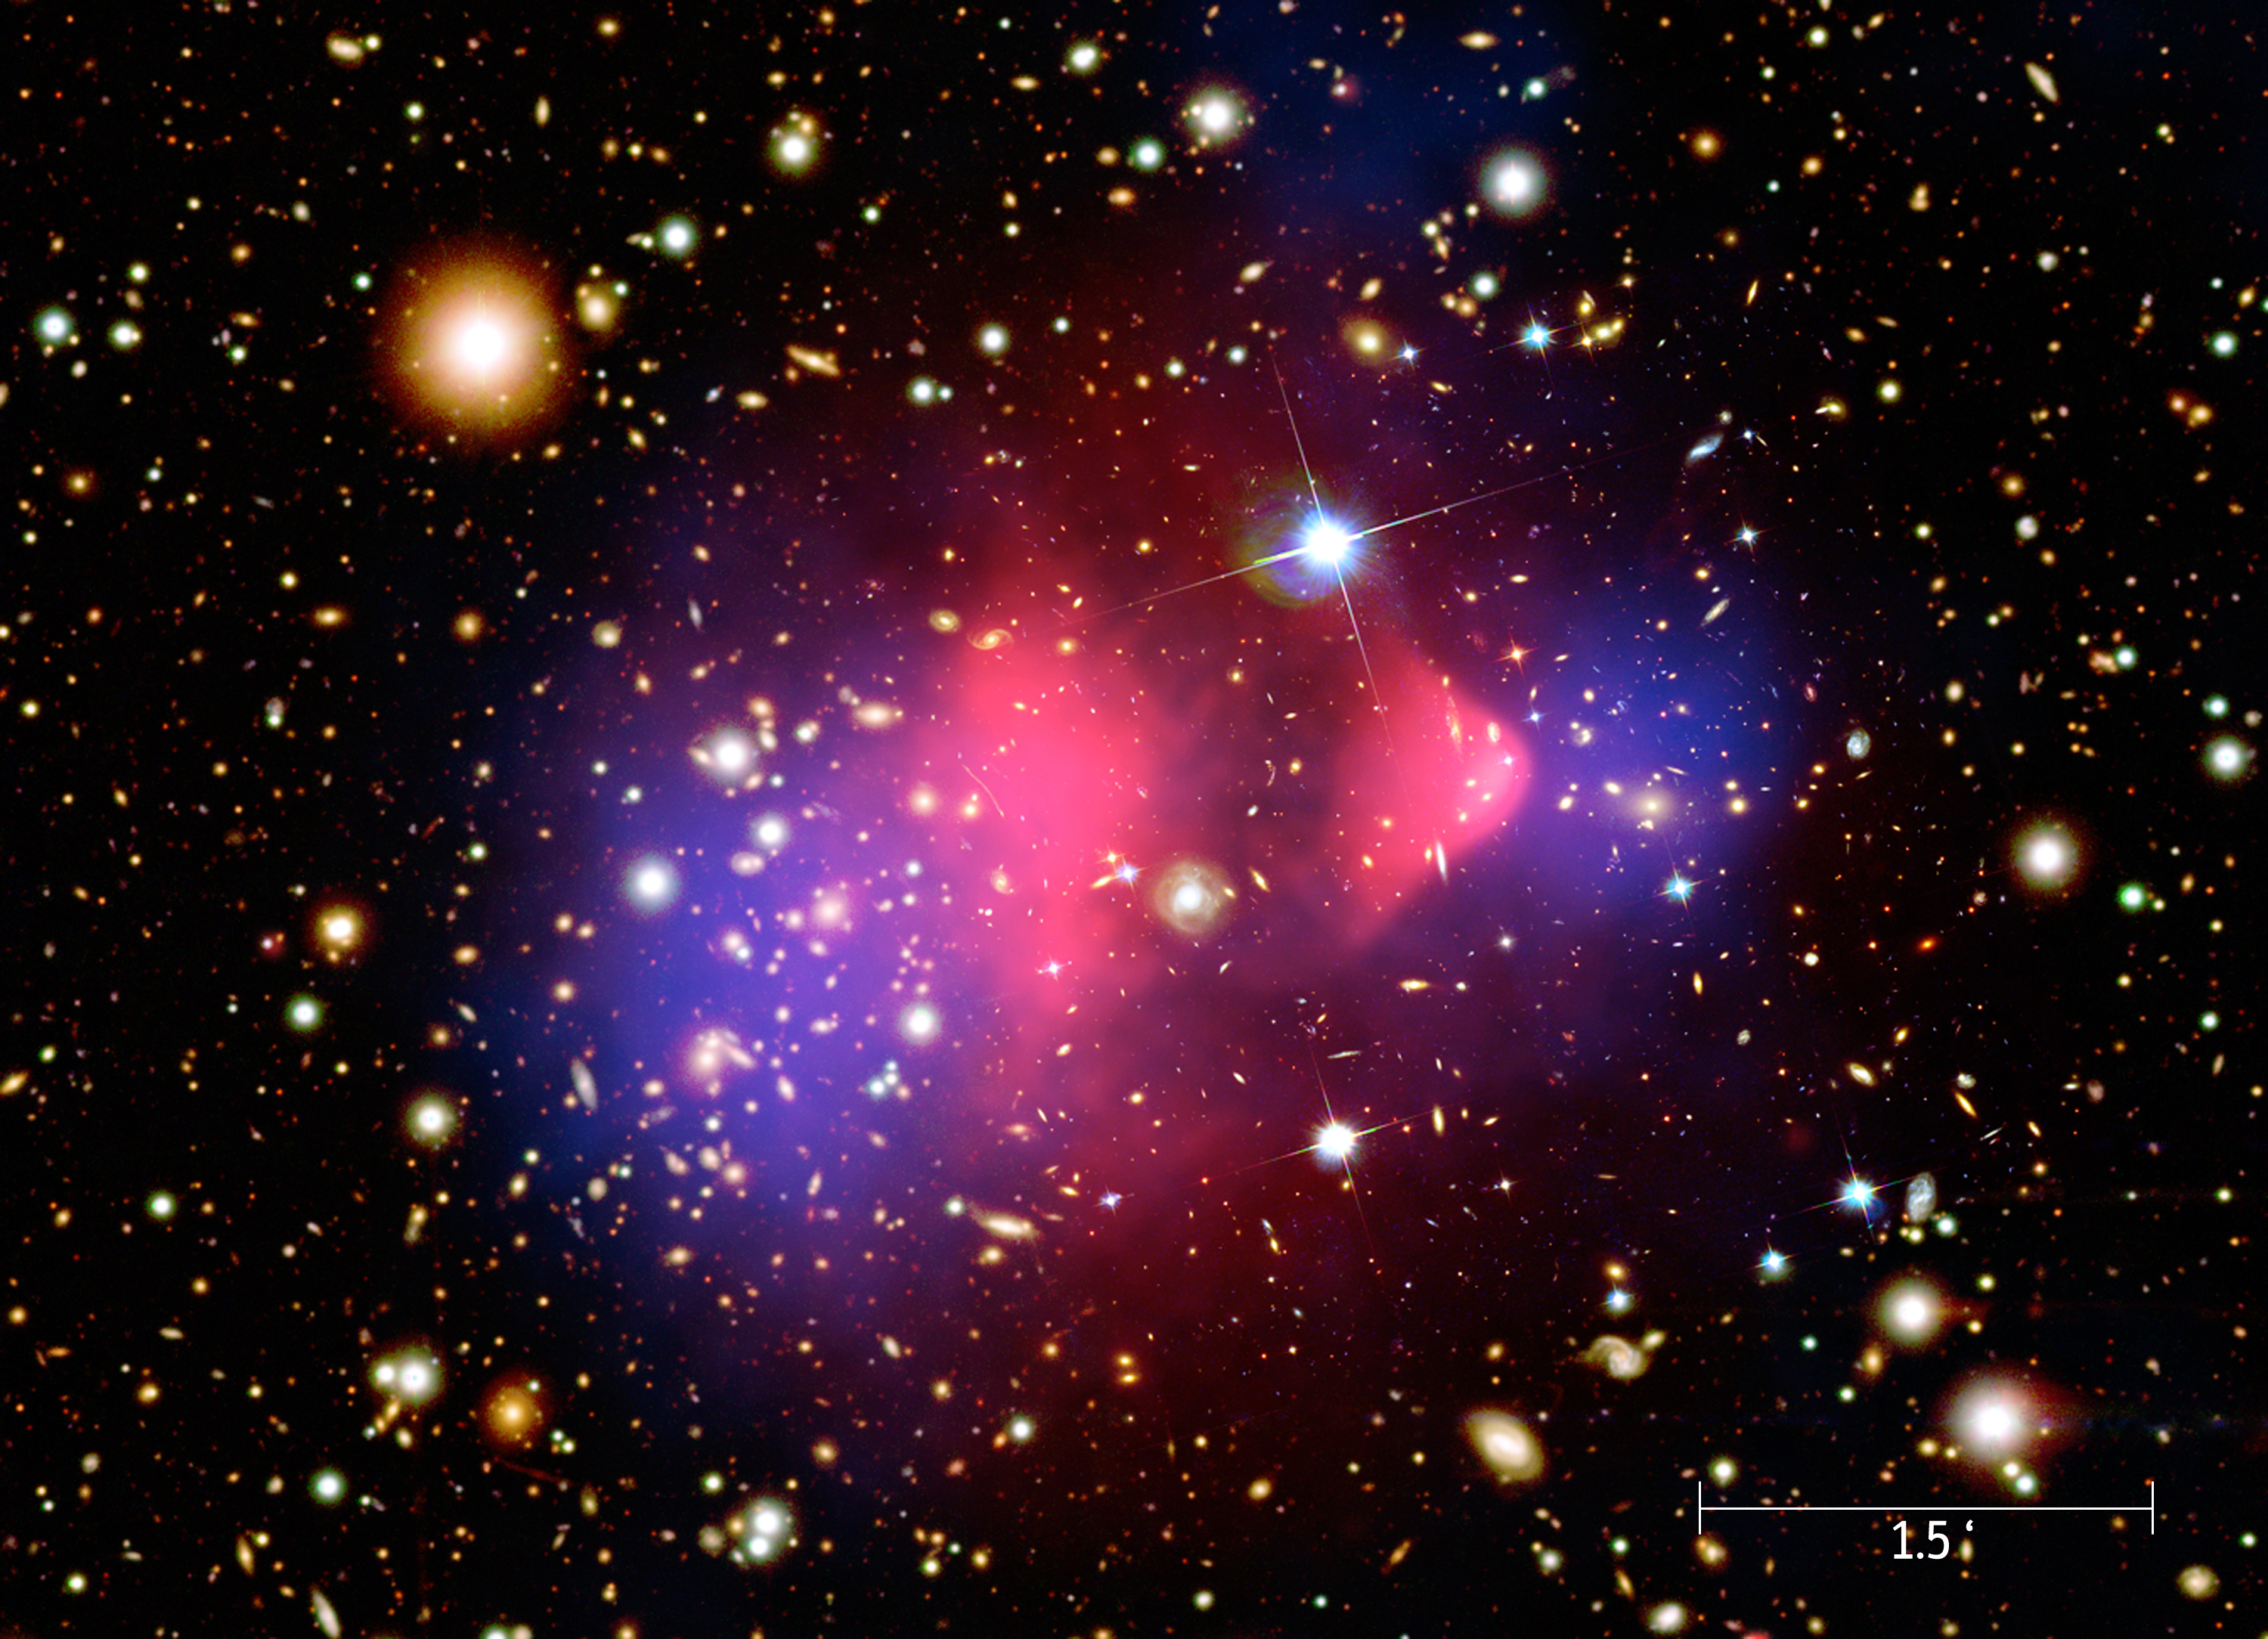
\includegraphics[width=\textwidth]{%
          ../figures/intro/bullet-cluster.jpg
        }
        \caption{Gravitational lensing (blue) and infrared (pink) observations
        show mass in different places!}
      \end{figure}
    \end{column}
  \end{columns}
\end{frame}

\note[itemize]{
\item One of the phenomena the SM doesn't account for is DM
\item We know it exists
}

\begin{frame}{Thermal Relic Dark Matter}
  \begin{block}{Narrow Wealth of Possibilities}
    Make the simple assumption that \ac{dm} has always been here.
  \end{block}
  \vfill
  \begin{figure}
    \centering
    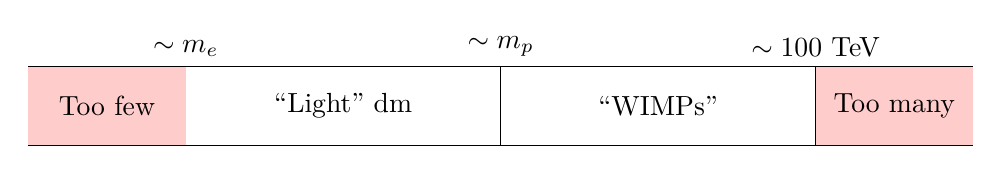
\begin{tikzpicture}
    % horizontal top/bottom lines
    \draw (0,0) -- (12,0);
    \draw (0,1) -- (12,1);
    % dividing lines along with relevant scale markers
    \draw (2,0) -- (2,1) node[above] {$\sim m_e$};
    \draw (6,0) -- (6,1) node[above] {$\sim m_p$};
    \draw (10,0) -- (10,1) node[above] {$\sim100~$TeV};
    % fill non-thermal ranges with light red
    \fill [red!20!white] (0,0) rectangle (2,1);
    \fill [red!20!white] (10,0) rectangle (12,1);
    % labels offering descriptions of ranges inside the boxes
    \node at (1,0.5) {Too few};
    \node at (4,0.5) {``Light'' \gls{dm}};
    \node at (8,0.5) {``WIMPs''};
    \node at (11,0.5) {Too many};
\end{tikzpicture}
    \caption{Mass scale of Thermal Relic \ac{dm}.
      The regions in red are excluded by applying the thermal relic assumption
      to our observations of the universe's early evolution.}
    \label{fig:dm-mass-scale}
  \end{figure}
  \boldcol{UMNSunny}{Both LDMX and HPS are searching for production of Light DM with electrons.}
\end{frame}

\ssection{LDMX}{ldmx}

\ssection{HPS}{hps}

\begin{backup}

\end{backup}

\end{document} 
